% The exact author's Elsevier CAS v2.4 class is copied by the build.
\documentclass[a4paper,fleqn]{cas-dc}
\usepackage[authoryear,longnamesfirst]{natbib}
\usepackage{amsmath,amssymb,mathtools,booktabs,graphicx,url}
\usepackage{hyperref}
\hypersetup{colorlinks=true,urlcolor=blue,linkcolor=blue,citecolor=blue}
\newcommand{\R}{\mathbb R}
\begin{document}
\let\WriteBookmarks\relax
\def\floatpagepagefraction{1}
\def\textpagefraction{.001}
\shorttitle{Jerk-aware PLS on observed vehicle trajectories}
\shortauthors{Espino-Montelongo and Cort\'es-Toto}
\title[mode=title]{Smoothness-indexed penalized trend estimation on measured vehicle trajectories: jerk, conditional extrapolation and selection-method comparison}
% Provisional author attribution, pending coauthor approval.
\author[1]{Heriberto Espino-Montelongo}
\author[1]{Daniela Cort\'es-Toto}
\affiliation[1]{organization={Universidad de las Am\'ericas Puebla},city={San Andr\'es Cholula},state={Puebla},country={Mexico}}
\begin{abstract}
We apply finite-difference penalized least squares to real, noisy vehicle-position data for which third differences have an interpretable connection to jerk. Five camera-derived longitudinal vehicle segments from the Federal Highway Administration NGSIM US-101 dataset are selected deterministically and sampled at 10 Hz. A normalized smoothness coordinate $S\in[0,1]$ controls polynomial trend regularization for orders $d=1,2,3,4$. Five classical selectors and two mean-difference policies are compared through strictly chronological observations held out for the next 0.5, 1, and 2 seconds; constant-velocity, constant-acceleration and Savitzky--Golay extrapolations provide physical baselines. We explicitly append a local polynomial continuation to the fitted PLS trend: forecasting is not an intrinsic output of PLS. Seven numerical implementations are compared separately for fitting cost and agreement. No future information enters selection, no synthetic data or noise are injected, and no ground-truth jerk measurement is claimed. This is an illustrative and falsifiable physical-data case study rather than a vehicle-control guarantee.
\end{abstract}
\begin{keywords}
Smoothness-indexed trend \sep jerk \sep real-world observations \sep NGSIM \sep penalized least squares \sep forecasting \sep numerical validation
\end{keywords}
\maketitle
\section{Introduction}
Vehicle longitudinal position is an unusually concrete application of high-order trend extraction: velocity, acceleration and jerk are its first, second and third temporal derivatives. The US Federal Highway Administration's Next Generation Simulation (NGSIM) dataset reports camera-derived vehicle positions every 0.1 seconds \citep{fhwa2016}. Earlier vehicle-trajectory research emphasizes that estimating acceleration from these observations magnifies measurement noise \citep{thiemann2008}; third derivatives amplify it further. This offers an interpretable reason to consider a $d=3$ difference penalty rather than choosing the ubiquitous quadratic-difference $d=2$ merely by tradition.

We study the PLS model of \citet{guerrero2007}, its trace-based smoothness index \citep{guerrero2008} and classical tuning criteria \citep{cortes2017}. The numerical-reliability and computational-complexity companions address generic spectral algorithms; this third paper is an independent, intentionally modest empirical case study. The question is whether smoothness-indexed PLS yields useful historical trends and how an \emph{explicitly separate} local continuation behaves when compared with measured future positions.

The dataset supplies physical position, but not independently measured latent truth or jerk. We never label a smooth jerk plot as the driver's actual acceleration derivative, do not add simulated noise, and distinguish interpolation, selection, extrapolation and out-of-sample verification.

\subsection{The noise amplification motivating third-order smoothing}
If measurement noise $\varepsilon_t$ has independent variance $\sigma_\varepsilon^2$, third forward differentiation uses stencil $(-1,3,-3,1)$, hence
\begin{equation}\label{eq:noise}
\operatorname{Var}\!\left(
\frac{D_3\varepsilon_t}{(\Delta t)^3}\right)
=\frac{20\sigma_\varepsilon^2}{(\Delta t)^6}.
\end{equation}
With $\Delta t=0.1$\,s, direct third differences can be extremely unstable. Equation~\eqref{eq:noise} is a conditional mathematical illustration, not an empirical noise-variance estimate: camera-tracking errors may be temporally correlated. Regularization suppresses variation but can bias sudden real changes in jerk. Thus plotted derivatives remain \emph{estimates}, not ground truth.

\section{Observed data and reproducible design}\label{sec:method}
\subsection{Camera-derived NGSIM US-101 longitudinal tracks}
The source is the US DOT/Federal Highway Administration NGSIM vehicle trajectory dataset (DOI: 10.21949/1504477) \citep{fhwa2016}. Its \texttt{Local\_Y} field is the longitudinal front-center vehicle coordinate, recorded in feet; \texttt{Global\_Time} is in milliseconds. We convert feet to meters exactly by 0.3048 and use elapsed time since each segment begins. The official dataset indicates CC BY-SA 3.0; extracted position subsets carry attribution and immutable hashes.

Data are downloaded directly from the USDOT Socrata API using a fixed query for US-101 vehicle identifiers 1--20. After sorting by vehicle and timestamp, a 100-ms gap splits track segments. In deterministic ascending order, the first five segments meeting minimum duration (200 points), displacement (20\,m), and conservative gross-quality thresholds are kept, without looking at forecast accuracy. The original vehicle identifiers may occur in several distinct recording periods; we retain track start timestamps to distinguish them. The complete extraction rule and source SHA-256 digests reside with the research scripts. Raw positions, rather than an already smoothed NGSIM derivative series, are the input.

The windows contain $n=80$ consecutive observations (8\,s), with prediction origins at segment indices 95, 140 and 185. Futures of $h=5,10,20$ frames (0.5, 1 and 2\,s) are withheld chronologically. The 15 origin windows overlap within five recorded segments. Observed held-out position is the error target, \emph{not} unavailable latent noise-free position or actual jerk; aggregate error scores are descriptive and not independent-sample confidence intervals.

\subsection{Smoothness-indexed quadratic trend}
For forward differences $D_d$ with $d\in\{1,2,3,4\}$, and fixed numeric mean of differences $\mu$, consider
\begin{equation}\label{eq:pls}
\widehat\tau_{\lambda,\mu}=
\arg\min_{\tau\in\R^n}\Bigl\{
\|y-\tau\|_2^2+
\lambda\|D_d\tau-\mu\mathbf1\|_2^2
\Bigr\}.
\end{equation}
If $\delta_j>0$ are the $n-d$ positive eigenvalues of $D_d^\top D_d$, the normalized degree-of-smoothing index is
\begin{equation}\label{eq:S}
S_d(\lambda)=\frac1{n-d}\sum_{j=1}^{n-d}
\frac{\lambda\delta_j}{1+\lambda\delta_j}\in[0,1].
\end{equation}
It is continuous and strictly increasing for $\lambda>0$, and independent of observed $y$ and fixed $\mu$. We invert $S$ once on the shared 16-point grid, including exact $S=0$ and $S=1$ endpoints, then reuse penalties across methods. No independently spaced log-$\lambda$ grid is a competitor here.

For $d=3$, the finite difference $D_3\tau_t$ divided by $(\Delta t)^3$ approximates physical jerk of a position signal. At $S=1$, fixed $\mu=0$ produces a quadratic trend (constant acceleration), whereas a fixed $\mu\ne0$ produces a cubic trend with approximately constant nonzero jerk. At finite $S$, the estimated third differences can vary over time. The two investigated policies are fixed $\mu=0$ and training-only plug-in $\widehat\mu=\operatorname{mean}(D_dy_{\rm train})$. Conditional CV scores for the latter do not re-estimate $\mu$ after each observation deletion, so cannot be interpreted as exactly refitted LOOCV.

\subsection{Five smoothing criteria}
On each training window and difference order, we minimize ordinary fixed-$\mu$ observation-deletion CV, generalized CV (GCV), AICc, residual-based BIC and Gaussian profiled marginal likelihood (ML) over the same bounded $S$ candidates. Residual BIC is explicitly restricted to $S\ge0.10$ because its unrestricted interpolation boundary is ill-posed; this is a sensitivity choice, not a theoretical correction. The Gaussian criterion profiles observation variance in a variance-components model with $\lambda=\sigma_\varepsilon^2/\sigma_\eta^2$, treating the polynomial nullspace as a nuisance component. A plug-in $\widehat\mu$ is not joint ML estimation of all variance and mean parameters. As a result, the criterion rows describe \emph{distinct in-sample selectors}, not directly comparable likelihood functions.

\subsection{Extrapolating a trend is a separate forecasting heuristic}
The public PLS fitting API estimates only the observed-period trend. For every selected fit, we use the final 25 smoothed points and fit a local polynomial of degree $d-1$ after removing the particular solution $\mu\binom{t}{d}$, then extrapolate that polynomial and add the particular solution back at future indices. This imposes the local limiting-$d$ polynomial pattern but \emph{is not} a model-based predictive distribution or an intrinsic TrendEstimation forecasting algorithm. It can fail when the next driver action changes acceleration.

All methods receive identical held-out future positions. Physical comparators are 20-point local linear (constant-velocity) extrapolation, 30-point local quadratic (constant-acceleration) extrapolation, and a 21-point order-three Savitzky--Golay smoother followed by a 20-point local linear continuation \citep{savitzky1964}. Forecast RMSE is the square root of mean squared position errors in meters; MAE is likewise in meters.

\subsection{Separately comparing numerical implementations}
On the same recorded training windows at $d=3$, $S=0.90$, with both $\mu$ policies, we evaluate seven pathways: full shift-free SVD, fresh dense solve, dense Cholesky, general banded LU, banded Cholesky, symmetric Gram eigendecomposition and dual SVD. Each has three within-run wall-clock repetitions and a numerical fit discrepancy measured against full SVD. These are \emph{one-fit} timings; they do not include the computational cost of evaluating full CV/GCV/AICc/BIC/ML grids. Any failed or nonfinite pathway is reported as unavailable rather than treated as a fast winner.

\section{Real-data results and comparisons}
\subsection{One held-out trajectory and its fitted jerk}
Figure~\ref{fig:forecast} shows a predeclared chronological cutoff of the first real US-101 vehicle segment. The original recorded positions, smooth in-sample trend and extrapolated future are shown separately. Predictions are made without seeing the future; the PLS fit itself contains no built-in forecast model.
\begin{figure*}[t]\centering
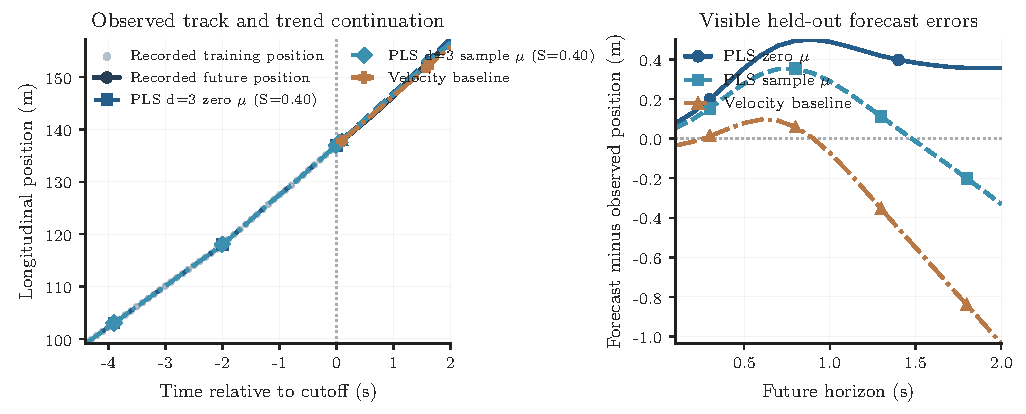
\includegraphics[width=\textwidth]{figures/heldout_forecast.pdf}
\caption{Measured training and future longitudinal position, with $d=3$ GCV-selected PLS trends under zero and training-derived means and their local-polynomial continuations. The observed future is withheld during estimation.}
\label{fig:forecast}
\end{figure*}
Third differences have meaningful units only after dividing by the cubed 0.1-s sampling interval. Figure~\ref{fig:jerk} illustrates strong differentiation noise in the original position and the smaller, regularized jerk proxy of the selected PLS trend. Neither derivative is independently observed true jerk.
\begin{figure*}[t]\centering
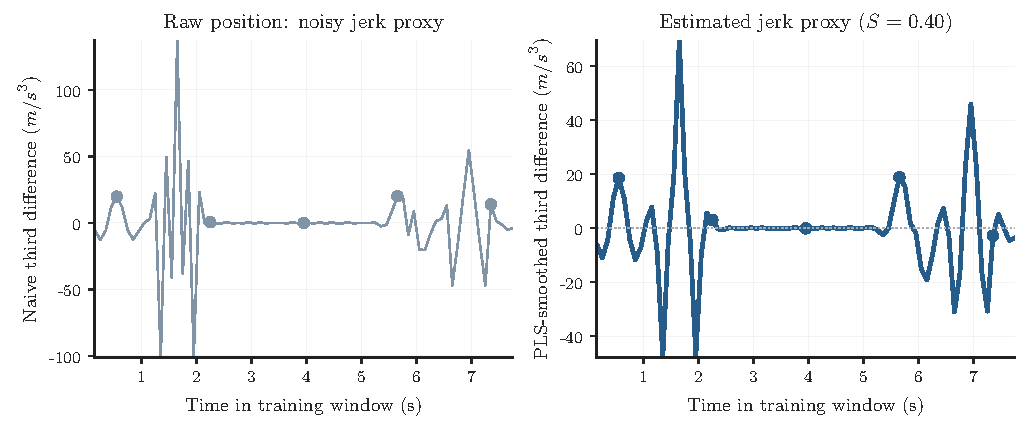
\includegraphics[width=\textwidth]{figures/jerk_comparison.pdf}
\caption{Direct and PLS-smoothed third differences of the same measured US-101 position segment. Panel axes have different scales; reduced amplitude after smoothing does not establish physical accuracy.}
\label{fig:jerk}
\end{figure*}

\subsection{Five criteria, four orders and both mean policies}
Table~\ref{tab:forecast} reports genuinely held-out position RMSE at the one-second horizon for the main PLS orders and physical baselines; Figure~\ref{fig:criteria} provides the complete $d=1,\ldots,4$ by five-criterion comparison for both $\mu=0$ and training-data plug-in mean of differences. Every method is scored against the same recorded future positions, not an unavailable noise-free latent trend.
% GENERATED FROM REAL NGSIM HOLDOUT RESULTS; DO NOT EDIT
\begin{table*}[t]
\caption{Out-of-sample position RMSE in meters at a one-second horizon (15 chronological track-origin windows). The five selection criteria used the same normalized S candidates, except restricted BIC ($S\ge0.10$). The data-derived mean policy changes model specification and does not yield exact refitted LOOCV.}
\label{tab:forecast}\centering
\begin{tabular}{lrrrr}
\toprule
Selector & $d=2,\ \mu=0$ & $d=3,\ \mu=0$ & $d=3,\ \widehat\mu$ & $d=4,\ \mu=0$ \\
\midrule
CV & 0.600 & 0.583 & 0.475 & 0.933 \\
GCV & 0.600 & 0.583 & 0.475 & 0.933 \\
AICc & 0.600 & 0.583 & 0.475 & 0.932 \\
Restricted BIC & 0.600 & 0.583 & 0.475 & 0.933 \\
Profile ML & 0.600 & 0.583 & 0.475 & 0.932 \\
\midrule
Velocity baseline & \multicolumn{4}{c}{0.547} \\
Acceleration baseline & \multicolumn{4}{c}{0.626} \\
Savitzky--Golay velocity & \multicolumn{4}{c}{0.543} \\
\bottomrule
\end{tabular}
\end{table*}

% AUTO-GENERATED REAL-DATA RESULTS
For $d=3$, GCV-selected PLS continued from 80 observed frames gives
0.583\,m RMSE under fixed $\mu=0$ and 0.475\,m
when the training-only sample mean of third differences is plugged in.
The corresponding constant-velocity and constant-acceleration baselines
give 0.547\,m and
0.626\,m, respectively.
The comparison is illustrative; highly similar criterion-level scores
do not indicate five independent demonstrations of superiority.

\begin{figure*}[t]\centering
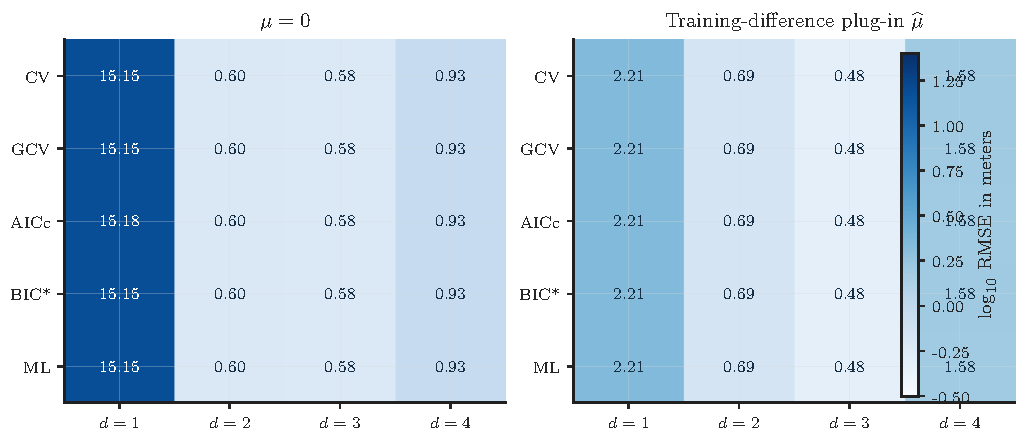
\includegraphics[width=\textwidth]{figures/criterion_heatmap.pdf}
\caption{Held-out one-second position RMSE in meters (printed values) across all four orders and all five criteria; $\mu$ policies are separated. Colors represent log-RMSE for display, not significance. BIC was restricted to $S\ge0.10$.}
\label{fig:criteria}
\end{figure*}

\subsection{Extrapolation horizon and physical baselines}
The experiment evaluates $h=5,10,20$ future 100-ms frames rather than labeling in-sample fitted values as forecasts. Figure~\ref{fig:horizons} compares selected $d=2,d=3$ PLS continuations with constant-velocity, constant-acceleration and Savitzky--Golay physical baselines. Smooth historical fits can extrapolate poorly if acceleration changes abruptly.
\begin{figure*}[t]\centering
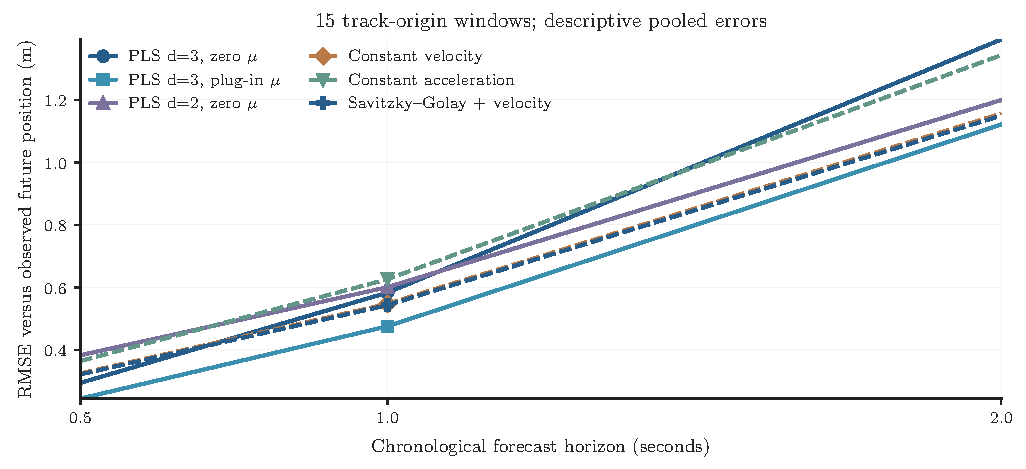
\includegraphics[width=\textwidth]{figures/forecast_horizons.pdf}
\caption{Chronological 0.5, 1 and 2-second position errors across 15 overlapping track-origin windows; comparisons use future measured camera-derived position, not latent truth.}
\label{fig:horizons}
\end{figure*}

\subsection{All seven numerical fitting pathways}
For completeness, we separately compare shift-free full SVD, dense solve, dense Cholesky, general banded LU, banded Cholesky, symmetric Gram eigendecomposition and dual SVD using the same observed windows at $d=3,S=0.9$. Table~\ref{tab:solver} and Figure~\ref{fig:backend} give fit-only median timings and relative fit discrepancies against SVD. This is a numerical calculation study, not a five-criterion selection runtime study or a measurement of physical jerk accuracy.
% GENERATED FROM REAL NGSIM FITTING BENCHMARK
\begin{table*}[t]
\caption{Same observed position windows, seven fit-only numerical backends, $d=3$, $S=0.90$. Median runtime is across 10 model/mean cases, each with three within-run timing repetitions; maximum relative fit error uses full SVD as the numerical baseline. Hardware-specific values do not predict criterion-selection timing.}
\label{tab:solver}\centering
\begin{tabular}{lrrr}\toprule
Solver & Valid cases & Median fit time (ms) & Max.\ relative discrepancy \\
\midrule
Full SVD & 10 & 0.0423 & 0.00e+00 \\
Dense LU & 10 & 0.0566 & 1.38e-12 \\
Dense Cholesky & 10 & 0.0401 & 1.65e-12 \\
Banded LU & 10 & 0.2047 & 1.27e-12 \\
Banded Cholesky & 10 & 0.0192 & 1.07e-12 \\
Gram eigendecomp. & 10 & 0.4226 & 3.26e-12 \\
Dual SVD & 10 & 0.6657 & 2.62e-17 \\
\bottomrule
\end{tabular}
\end{table*}

\begin{figure*}[t]\centering
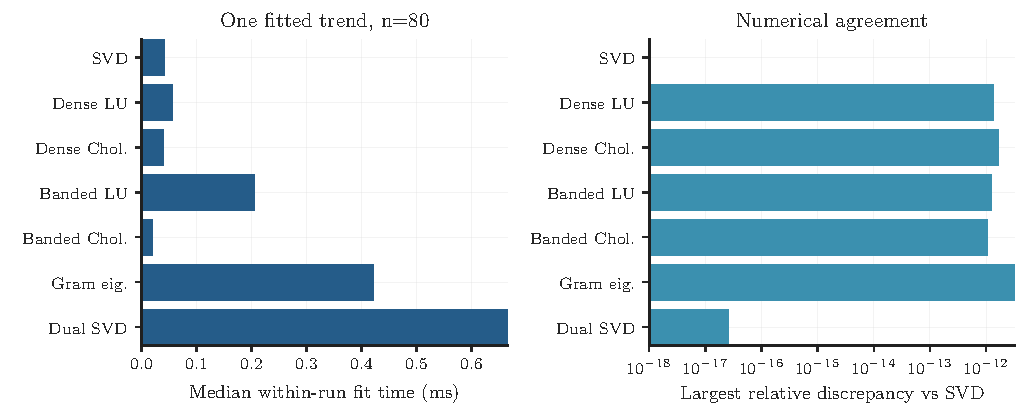
\includegraphics[width=\textwidth]{figures/backend_comparison.pdf}
\caption{Fit-only elapsed milliseconds and relative numerical discrepancies on real recorded positions under two $\mu$ policies. Numerical fit differences are not statistical forecast errors.}
\label{fig:backend}
\end{figure*}

\section{Discussion and conclusions}
The observed vehicle positions illustrate why model difference order, reference mean and extrapolation method must be kept distinct. For a position series, $d=3$ has a direct relation to the third temporal derivative---jerk---but neither the raw third difference nor its smoothed counterpart is an independent physical reference signal. A smooth-looking jerk series can still underrepresent actual sudden driver maneuvers.

The normalized coordinate $S\in[0,1]$ solves an important interpretability problem: it has consistent meaning across difference orders, regardless of the scale of the internal penalty $\lambda$, and its inverse map does not depend on the fixed mean of differences. The user-facing selection grid is always expressed in $S$, not an arbitrary independently sampled log-$\lambda$ coordinate. Pretranslation and reuse are computational optimizations, not new statistical models.

The principal practical conclusion must be qualified. A favorable GCV-selected $d=3$ one-second held-out result in this restricted sample is a descriptive illustration and cannot establish generalized vehicle-prediction superiority. The fifteen training/holdout origins overlap within five recorded segments and do not justify naive independent-window inference. Selection criteria may yield nearly identical smooth trends, and the observed position itself includes unmeasured camera noise.

The training-data mean-difference policy uses no future information, but CV scores computed conditionally on that plug-in mean are not exact re-estimated LOOCV. Profiled Gaussian marginal likelihood requires variance assumptions; it is not point-estimator MLE for $\tau$ or joint ML estimation of $\mu$. Restricted residual BIC remains an exploratory constrained criterion because the original unrestricted interpolation boundary is mathematically pathological.

Our extrapolation is an explicit local polynomial applied to the historical PLS fit. It is \emph{not} a predictive distribution, and it cannot anticipate unobserved changes in acceleration, traffic interactions or lane changes. Future research requires independent maneuvers, substantially more vehicles, genuine measurement-error characterization, and a dedicated dynamic/state-space forecast comparison. The seven fitting backends are benchmarked for single-curve cost and numerical agreement; complete-selection runtime and independent multiprecision accuracy are addressed by companion studies.

\section*{Reproducibility and data rights}
The US DOT/FHWA NGSIM dataset (DOI: 10.21949/1504477) is credited as the sole source of observed positions; the dataset portal identifies a CC BY-SA 3.0 license. Source query and extraction rules, tracked vehicle identifiers, segment starting timestamps, immutable checksums, chronological forecast rows, solver diagnostics, source-generation scripts and editable PGF vector figures are preserved under the case-study directory. The original official-position subset has not been artificially contaminated or pre-smoothed. Figure-derived jerk is explicitly estimated rather than observed.

\section*{Declarations}
This is an illustrative research draft. Authorship, correspondence, funding, conflicts and any journal submission require coauthor review and agreement.

\bibliographystyle{cas-model2-names}
\bibliography{references}
\end{document}
